% -----------------------------------------------
% Template for ISMIR 2013
% (based on earlier ISMIR templates)
% -----------------------------------------------
%
% \usepackage{ismir2013,amsmath,cite}
% \usepackage{graphicx}
% %custom packages
% \usepackage{footnote}
% \usepackage{color}
% \usepackage{multirow}
% \usepackage{xcolor}
% \usepackage{multirow}
% \usepackage{makecell}
% \usepackage{textcomp}
% \usepackage{subfigure}
% \usepackage{amssymb}
% \usepackage{booktabs}
% \usepackage{siunitx}
% \usepackage{colortbl,array}
% \usepackage{url}
% \makeatletter
% \g@addto@macro{\UrlBreaks}{\UrlOrds}
% \makeatother
% \usepackage{tikz}
% \usetikzlibrary{arrows}
% \usepackage{pgfplots}
% \pgfplotsset{compat=1.8}
% \usepgfplotslibrary{statistics}
% \usetikzlibrary{patterns}
% \usepackage{anyfontsize}

Internet experiments in the fields of music perception and music information retrieval are becoming more and more popular. However, not many Internet experiments are compared to laboratory experiments, the consequence being that the effect of the uncontrolled Internet environment on the results is unknown.
In this paper the results of an Internet experiment with 1168 participants are compared to those of the same experiment with 62 participants but previously conducted in a controlled environment. The comparison of the Internet and laboratory results enabled us to make a point on whether the Internet can be used for our experiment procedure. The experiment aimed to investigate the listeners ability to correctly estimate the number of instruments being played back in a given excerpt of music. The participants listened to twelve short classical and pop music excerpts each composed using one to six instruments. For each music excerpt the participants were asked how many instruments they could hear and how certain they were about their estimation.
%
\section{Introduction}\label{sec:introduction}
%For developing source separation algorithms, knowing the maximum number of instruments humans are able to identify could be helpful. E.~g. this number can be used as a target value which the algorithm has to outperform when the algorithm has to be better than the auditory system of humans.

In psychoacoustics, a sequence of sounds grouped by the auditory system is known as an ``auditory stream'' which was coined by Bregman and Campbell\cite{Bregman1971}. In the past decades, a lot of experimental work related to ``auditory streams'' has been done\cite{bregman90}. A majority of these experiments were psychoacoustically motivated, e.~g. the stimuli used were mostly of simple type like sinusoids or noises. Especially from a psychoacoustic point of view, music is a very complex sound signal which contains high-level information (e.~g. instrumentation and song lyrics). When listening to music, this high-level information is also mentally processed by humans. For developing auditory models, it could be helpful to know the maximum number of instruments humans are able to estimate when listening to music.

For many types of music perception experiments such as estimating the number of instruments, it is essential that the selected participants represent a large population. As recent research in cross-cultural music perception and cognition reveals: The perception of music is dependent on the origin of people\cite{Stevens2012}. Besides the cultural background, other aspects like their profession might have an influence when estimating the number of instruments being played back, e.~g. musicians might recognize instruments much more easily since they are in touch with instruments in their everyday life. One of the advantages of Internet experiments (also called web-based experiments or web experiments) is that it is easier to gather participants with different backgrounds and from different regions than in laboratory experiments. For a summary of benefits and disadvantages of Internet experiments see \cite{Reips2002}. In music perception a major argument against Internet experiments is that there is no control about the environment. With the spreading of mobile devices with Internet connections this argument becomes more apparent, since the environment of the participants can range from a quiet place at home to a noisy place outside.

By comparing the results of the Internet experiment presented in this paper to the results of the same experiment but previously conducted in a controlled environment\cite{Stoter2013}, we contribute to answering the research question, whether the Internet can be used for experiments in music perception. Furthermore, subpopulations like headphones-users and loudspeaker-users are examined whether they lead to more reliable responses.

\section{Related Work}\label{sec:related_work}
The ability of estimating the number of instruments is probably related to the ability of auditory stream segregation. An overview of auditory stream segregation in general is given by Bregman\cite{bregman90} and Wang and Brown\cite{wang2006}.

In 1989, Huron conducted a musically motivated experiment related to stream segregation\cite{Huron1989}. In his experiment he asked the participants for the number of voices in excerpts of organ music. Huron defined a voice as a single ``line'' of sound, more or less continuous, that maintains a separate identity in a sound field or musical texture (an overview of voice definitions is given by Cambouropoulos\cite{Cambouropoulos2008}). Huron came to the conclusion that the number of correctly identified voices is up to three. Based on Hurons work, we carried out an experiment where we asked musicians and non-musicians how many instruments they could hear in short pieces of music\cite{Stoter2013}. In contrast to Huron we addressed a more general case where voices are played by different instruments and not only by organ. In Huron's experiment the responses of the participants were time-varying for each stimulus. Another difference is that in Huron's experiment all six participants except one had a musical background whereas our experiment was also attended by a large group of non-musicians.

It has been becoming more and more popular to use the Internet for experiments in music or auditory perception. One of the first auditory experiments were conducted by Welch and Krantz\cite{Welch1996} in 1996. A web experiment related to MIREX tasks using \emph{Amazon Mechanical Turk} has been conducted by Lee \cite{lee2010}. An experiment with a large attendance was done by Salganik~\textit{et~al.}\cite{Salganik2006} in 2006. They had over 14.000 participants and examined the social influence on participants in an artificial music market. An overview of recent Internet experiments is given by Reips\cite{Reips2012}.

\section{Method}\label{sec:method}

\subsection{Stimuli}\label{sec:stimuli}
For the stimuli generation, MIDI files of music pieces from the RWC database\cite{rwc} were selected. The MIDI files were modified so that each file has a specific number of instruments being played back. Since the number of instruments being played back had to be as constant as possible, a so-called ``instrumental stationarity'' for each music piece was calculated. The ``instrumental stationarity'' is a measure that shows whether all instruments are played the whole time for a given start position and length. See \cite{Stoter2013} for the detailed equation of ``instrumental stationarity'' and more information about the stimuli generation. The RWC files were manually filtered a priori to exclude items dominated by lead instruments or singing voices. From the remaining items thirteen excerpts of MIDI files were selected with the help of the ``instrumental stationarity'' having one to six simultaneously playing instruments. Table~\ref{table:items} shows the selected excerpts including their instrumentation. The duration of each excerpt is around seven seconds. By cutting at note offsets we varied the lengths of the excerpts to make them semantically more meaningful. Six items (notated as C0**) belong to the classical Western music genre whereas the other items are of mixed genre.
\renewcommand{\arraystretch}{1.1}
\begin{table}[htb]
\center
\tiny
\begin{tabular}{c|r@{.}l|r@{.}l|p{3.8cm}|c}
\toprule[1.5pt]
RWC~ID & \multicolumn{2}{c}{Start~[s]} & \multicolumn{2}{c}{Dur.~[s]} & Instrumentation & $\sum$\\
\midrule
\hline
J021 & 46 & 5 & 6 & 6 & Piano, Contrabass~(pizz.) and Trumpet & 3\\
\hline
\hline
C001 & 0&0 & 9&0 & Bassoon & 1  \\
G047 & 35&3 & 8&3 & Violoncello & 1 \\
\hline
C016 & 0&9 & 7&6 & Viola and Violoncello & 2\\
G068 & 132&4 & 6&6 & Violin and Flute &  2\\
\hline
C018 & 240&4 & 5&4 & French~Horn, Piano and Violin & 3\\
G046 & 0&3 & 7&9 & Contrabass, Piano and Violoncello & 3\\
\hline
C013 & 5&6 & 6&0 & Flute, Viola, Violin and Violoncello & 4\\
G036 & 0&0 & 6&5 &  Acoustic~Guitar, Electric~Bass, Piano  and Violin & 4\\
\hline
C012 & 112&0 & 6&0 & Contrabass, Flute, Viola, Violin and  Violoncello & 5\\
G037 & 67&1 & 7&0 & Acoustic~Guitar, Contrabass~(pizz.), Flute, Piano and Tenor~Sax & 5\\
\hline
C001 & 147&8 & 6&0 & Bassoon, Clarinet, Contrabass, French~Horn, Oboe and Violin & 6\\
G028 & 17&5 & 6&5 & Electric~Bass, Electric~Guitar, Flute, Piano, Trombone and Trumpet & 6\\
\hline
\bottomrule[1.5pt]
\end{tabular}
\renewcommand{\arraystretch}{1}
\caption{Selected items from the RWC~Music~Database\cite{rwc}. Item \emph{J021} was used as training item.}
\label{table:items}
\end{table}
The MIDI excerpts were humanized and rendered by a sequencer software utilizing state-of-the-art commercial sampling products into WAV files. The rendered files were processed with convolutive reverb to match the original recordings. In informal listening tests the quality of the renderings was evaluated. In addition, participants did not give negative feedback about the artificialness of the items during the laboratory experiment. Additionally a loudness normalization was applied according to EBU-R128\cite{EBU2011}. To avoid spatial cues the files were downmixed to mono at 16~bit/44.1~kHz.

\subsection{Participants}
Participation in the experiment was done by visiting the experiment's website\footnote{{\scriptsize\url{http://www.audiolabs-erlangen.com/experiments/wice/}}}. The experiment was promoted in mailing lists, forums, social networks and by personal invitations. Most of the forums and mailing lists were audio-related. No material incentive was given to participants. For motivating the participants a high score was added to the experiment.

In total 1310 website visitors attended the experiment. We identified 115 of them as participants who did the experiment more than once by using a browser fingerprinting method (for more details in browser fingerprinting, see \cite{Eckersley2010}). In this case, only the first trial is used in the results analysis. Our browser fingerprinting method created a hash value by using the visitor's browser settings, e.~g. screen resolution and installed plugins. In addition, we excluded 27 participants since they gave at least one non-serious response. We defined responses with zero instruments (25~participants) and responses with more than 12 instruments (two participants) as invalid. After the screening we had 1168 valid participants.

The participants were asked by a questionnaire whether they have a professional background in audio, play at least one instrument (including singing) and are familiar with listening tests. Detailed information about the participants are described in Table~\ref{table:info_participants}.
\begin{table}[htb]
\center
\scriptsize
\renewcommand{\arraystretch}{1.2}
%\begin{tabular}{cr@{.}lr@{.}lr@{.}l}
\begin{tabular*}{0.45\textwidth}{c r@{ }l r@{ }l r@{ }l r@{ }l r@{ }l}
\toprule[1.5pt]
Total & \multicolumn{2}{c}{Age group} & \multicolumn{2}{c}{Musician} & \multicolumn{2}{c}{Professional} & \multicolumn{2}{c}{Headphones} \\
\midrule
1168 &  0  & [0-12]  & -   &  	   & -   &       & -   &       \\
 	 \cline{2-9} \rule{0pt}{10pt}
     & 110 & [13-19] & 74  & [yes] & 12  & [yes] & 5   & [yes] \\
     &     &         &	   &       &     &       & 7   & [no]  \\
     &     &   		 &     &       & 62  & [no]  & 30  & [yes] \\
     &     &         &	   &       &     &       & 32  & [no]  \\
     &     &   		 & 36  & [no]  & 0   & [yes] & -   &       \\
     &     &         &	   &       &     &       & -   &       \\
     &     &   		 &     &       & 36  & [no]  & 17  & [yes] \\
     &     &         &	   &       &     &       & 19  & [no]  \\
     \cline{2-9} \rule{0pt}{10pt}
     & 889 & [20-39] & 463 & [yes] & 128 & [yes] & 81   & [yes] \\
     &     &         &	   &       &     &       & 47   & [no]  \\
     &     &   		 &     &       & 335 & [no]  & 154  & [yes] \\
     &     &         &	   &       &     &       & 181  & [no]  \\
     &     &   		 & 426 & [no]  & 46  & [yes] & 31   & [yes] \\
     &     &         &	   &       &     &       & 15   & [no]  \\
     &     &   		 &     &       & 380 & [no]  & 164  & [yes] \\
     &     &         &	   &       &     &       & 216  & [no]  \\
     \cline{2-9} \rule{0pt}{10pt}
     & 143 & [40-59] & 98 & [yes] & 32  & [yes] & 22   & [yes] \\
     &     &         &	  &       &     &       & 10   & [no]  \\
     &     &   		 &    &       & 66  & [no]  & 31   & [yes] \\
     &     &         &	  &       &     &       & 35   & [no]  \\
     &     &   		 & 45 & [no]  & 8   & [yes] & 5    & [yes] \\
     &     &         &	  &       &     &       & 3    & [no]  \\
     &     &   		 &    &       & 37  & [no]  & 17   & [yes] \\
     &     &         &	  &       &     &       & 20   & [no]  \\
     \cline{2-9} \rule{0pt}{10pt}
     & 26  & [60+]   & 13 & [yes] & 6   & [yes] & 3    & [yes] \\
     &     &         &	  &       &     &       & 3    & [no]  \\
     &     &   		 &    &       & 7   & [no]  & 4    & [yes] \\
     &     &         &	  &       &     &       & 3    & [no]  \\
     &     &   		 & 13 & [no]  & 2   & [yes] & 2    & [yes] \\
     &     &         &	  &       &     &       & 0    & [no]  \\
     &     &   		 &    &       & 11  & [no]  & 5    & [yes] \\
     &     &         &	  &       &     &       & 6    & [no]  \\
\bottomrule[1.5pt]
\end{tabular*}
\caption{Information about the participants.}
\renewcommand{\arraystretch}{1}
\label{table:info_participants}
\end{table}

\subsection{Materials and Apparatus}\label{sec:materials}
The main functionality of the experiment's website was written in HTML5 and JavaScript. The website was tested for all major web browsers and optimized for mobile devices and desktop computers. The default file format for the stimuli was WAV. Since some browsers (e.~g. Internet Explorer) did not support WAV, MP3 (encoded with \SI{256}{kbits/s} CBR with Fraunhofer Encoder) was used as alternative file format. The alternative file format was only used when WAV was not supported by the browser.

\subsection{Procedure}\label{sec:procedure}
The experiment started on February the 15th, 2013 and lasted until March the 15th, 2013. %TODO the data was captured between... and ...

At first, participants filled out a short questionnaire. They were asked which audio setup they are using, whether they regularly play any musical instruments or do singing, have a background in professional audio, are familiar with listening tests and which age group they belong to.

After filling out the questionnaire, the participants did a short training. The purpose of the training was to familiarize the participants with the user interface and to give them the option to adjust the volume. The training had one stimulus with three instruments being played. The instruments were piano, bass and trumpet. The participants were told on the training page how many and which instruments are played back. During the training it was possible to listen to the stimulus unlimited times.

Followed by the training, the participants had to estimate the number of instruments being played in twelve stimuli. The experiment question was ``How many different instruments do you hear?". Participants could listen to each stimulus up to three times. In addition, they were asked how certain they were in their response. They could choose between ``uncertain'', ``certain'' and ``very certain''. The user interface is shown in Figure~\ref{figure:user_interface}.

\begin{figure}[htb]
	\centering
		\fbox{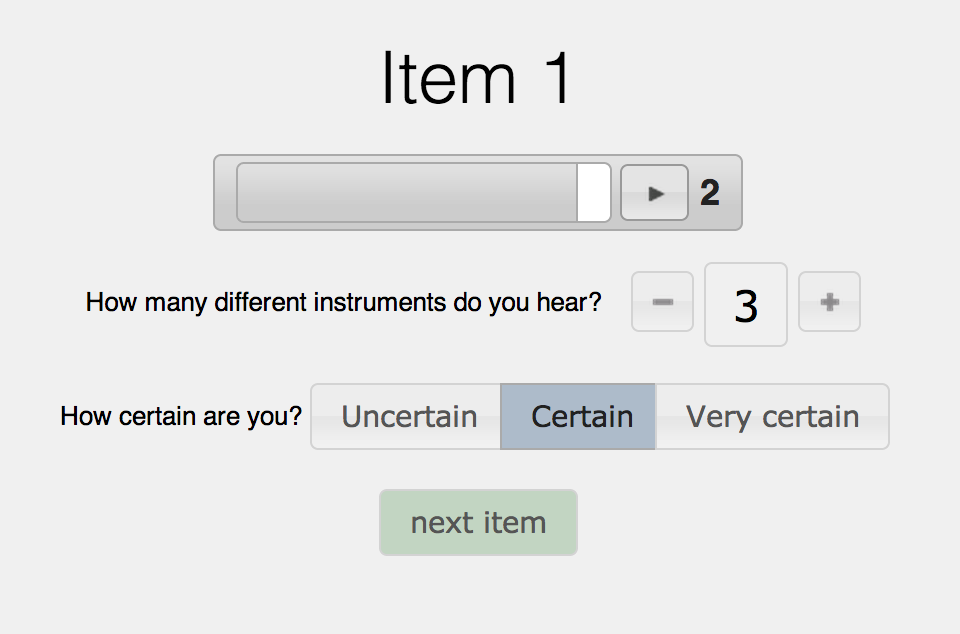
\includegraphics[width=2.8in]{Chapters/07_Analysis_Experiment/ismir/user_interface.png}}
	\caption{Experiment User Interface.}
	\label{figure:user_interface}
\end{figure}

After the participants estimated the number of instruments for all twelve stimuli, they were given a score based on their performance. Besides their personal score, a percentile rank showed how each participant performed compared to all the other participants.

\section{Results}\label{sec:results}

The independent variables are the number of instruments being played back ($\textit{Num}_{\mathrm{Inst}}$), whether a participant is musical ($\textit{Musical}$), professional in audio ($\textit{Professional}$) and which setup was used ($\textit{Setup}$). A participant is defined as musical ($\textit{Musical} = true$) when he or she is regularly playing an instrument (including singing). The same applies to being professional ($\textit{Professional} = true$) which is set when the participant responded that he or she is a professional in audio. The responses for the setup used can either be headphones ($\textit{Setup} = \textrm{`}headphones\textrm{'}$) or loudspeaker ($\textit{Setup} = \textrm{`}loudspeaker\textrm{'}$). The dependent variable is the participant's estimation of the number of instruments being played back ($\textit{Resp}$). A correct estimation is defined as
\begin{equation}
\label{equation:response_correct}
\textit{Resp}_{\mathrm{Correct}} =
\begin{cases}
0 & \text{if } \text{\textit{Num}}_{\mathrm{Inst}} \neq \text{\textit{Resp}}
\\
1 & \text{if } \text{\textit{Num}}_{\mathrm{Inst}} = \text{\textit{Resp}}
\end{cases}
\mathrm{.}
\end{equation}
Table~\ref{table:responses} shows the responses of the participants for all stimuli.
\tabcolsep=5.5pt
\begin{table}[t]
\tiny
\begin{tabular}{p{1cm}ccccccc}
\toprule[1.5pt]
 & \multicolumn{ 7}{c}{$\textit{Num}_{\mathrm{Inst}}$} \\
  \cmidrule(l){2-8}
 $\textit{Resp}$ & $I=1$ & $I=2$ & $I=3$ & $ I=4$ & $I=5$ & $I=6$ & n \\

 \midrule
 $R=1$ & \cellcolor[gray]{0.9} 2025 & 373 & 5 & 18 & 13 & 12 & 2446 \\
 \midrule
 $R=2$ & 298 & \cellcolor[gray]{0.9} 1642 & 810 & 736 & 451 & 382 & 4319 \\
 \midrule
 $R=3$ & 12 & 277 & \cellcolor[gray]{0.9} 1343 & 1145 & 1093 & 1069 & 4939 \\
 \midrule
 $R=4$ & 1 & 43 & 158 & \cellcolor[gray]{0.9} 386 & 645 & 680 & 1913 \\
 \midrule
 $R=5$ & 0 & 1 & 18 & 48 & \cellcolor[gray]{0.9} 120 & 155 & 342 \\
 \midrule
 $R=6$ & 0 & 0 & 1 & 3 & 12 & \cellcolor[gray]{0.9} 30 & 46 \\
 \midrule
 $R>6$ & 0 & 0 & 1 & 0 & 2 & 8 & 11 \\

 \midrule
 & \multicolumn{7}{c}{14016 responses (1168 participants $\cdot$ 12 items)} \\
\midrule[1pt]

Probability of $\textit{Resp}_{\mathrm{Correct}}$ & 0.87 & 0.70 & 0.57 & 0.17 & 0.05 & 0.01 &  \\

 \bottomrule[1.5pt]
\end{tabular}
\caption{Responses from the participants. The cells with a gray background represent correct estimations.}
\label{table:responses}
\end{table}
\tabcolsep=6pt

For testing hypotheses, a logistic regression model with the response variable $\textit{Resp}_{\mathrm{Correct}}$ and the predictor variables $\textit{Num}_{\mathrm{Inst}}$, $\textit{Musical}$, $\textit{Professional}$ and $\textit{Setup}$ was calculated.
The estimated coefficients, p-values and average marginal effects are shown in Table~\ref{table:data_web_lm}.
\tabcolsep=5.5pt
\begin{table}[t]
\center
\scriptsize
\begin{tabular}{p{1.5cm}ccccp{0.8cm}}
\toprule[1.5pt]
Coefficient & Estimate & Std. Error & z-value & p-value & Average Marginal Effects \\
\midrule
(Intercept) & 1.5015 & 0.06836 & 21.963 & \textless~2e-16 & 0.1886 \\
$\textit{Num}_{\mathrm{Inst}} = 2$ & -1.0293 & 0.07651 & -13.453  & \textless~2e-16 & -0.1293\\
$\textit{Num}_{\mathrm{Inst}} = 3$ & -1.6021 & 0.07463 & -21.466  & \textless~2e-16 & -0.2012\\
$\textit{Num}_{\mathrm{Inst}} = 4$ & -3.5674 & 0.08380 & -42.572  & \textless~2e-16 & -0.4481\\
$\textit{Num}_{\mathrm{Inst}} = 5$ & -4.8759 & 0.11290 & -43.188  & \textless~2e-16 & -0.6125\\
$\textit{Num}_{\mathrm{Inst}} = 6$ & -6.3061 & 0.19428 & -32.459  & \textless~2e-16 & -0.7922\\
$\textit{Musical} = true$ & 0.5266 & 0.04932 & 10.676  & \textless~2e-16 & 0.0661\\
$\textit{Professional} = true$ & 0.3306 & 0.06234 & 5.303  & 1.14e-07 & 0.0415\\
$\textit{Setup} = \textrm{`}headphones\textrm{'}$ & 0.1071 & 0.04823 & 2.220  & 0.0264 & 0.0135\\
\midrule
\multicolumn{6}{l}{(Dispersion parameter for binomial family taken to be 1)}\\
\multicolumn{6}{l}{Null deviance: 18816  on 14015  degrees of freedom}\\
\multicolumn{6}{l}{Residual deviance: 11036  on 14007  degrees of freedom}\\
\multicolumn{6}{l}{AIC: 11054}\\
\multicolumn{6}{l}{Number of Fisher Scoring iterations: 7}\\
\multicolumn{6}{l}{McFadden's Pseudo R-squared: 0.413}\\
\bottomrule[1.5pt]
\end{tabular}
\tabcolsep=6pt
\caption{Logit regression model for response variable $\textit{Resp}_{\mathrm{Correct}}$ calculated from the data obtained by the Internet experiment.}
\label{table:data_web_lm}
\end{table}
Average marginal effects in the regression model describe the increase in probability for correctly estimating the number of instruments when the predictor variable is increased by one level. Compared to the other coefficients the average marginal effect of $\textit{Setup} = \textrm{`}headphones\textrm{'}$ is very low. By using headphones instead of loudspeakers it is $1.35\%$ more likely to estimate the number of instruments correctly.

As expected, participants who play an instrument or do singing ($\textit{Musical} = true$) performed slightly better than non-musicians. According to the average marginal effect their chance of estimating the number of instruments correctly is $6.61\%$ more likely for all stimuli. A similar increase for estimating the number correctly ($4.15\%$) can be seen for participants being a professional in audio ($\textit{Professional} = true$).

The average marginal effects of $\textit{Num}_{\mathrm{Inst}}$ indicates up to which point humans are able to correctly estimate the number of instruments being played back. The average marginal effect of $\textit{Num}_{\mathrm{Inst}} = 2$ shows that it is $12.93\%$ less likely to estimate correctly when listening to two instruments instead of one instrument. Furthermore, in case of three instruments being played back the probability of estimating the wrong number increases to $20.12\%$. The highly negative average marginal effect of $-0.4481$ for $\textit{Num}_{\mathrm{Inst}} = 4$ indicates that it is becoming very unlikely for humans to estimate the number of instruments correctly compared to estimating the number of one to three instruments.

For a detailed analysis of the differences between the Internet experiment and the laboratory experiment in a controlled environment, a second logit regression model was calculated. This logit regression model includes the data of the previous experiment which has responses of 62 participants. Besides $\textit{Num}_{\mathrm{Inst}}$ an additional predictor variable $\textit{Environment}$ was added which can have the values $\textrm{`}web\textrm{'}$ or $\textrm{`}lab\textrm{'}$ (described in Table~\ref{table:data_both_lm}).
\begin{table}[t]
\center
\scriptsize
\begin{tabular}{p{1.5cm}ccccp{0.8cm}}
\toprule[1.5pt]
Coefficient & Estimate & Std. Error & z-value & p-value & Average Marginal Effects \\
\midrule
(Intercept) & 2.0226 & 0.11718 & 17.260 & \textless~2e-16 & 0.2590\\
$\textit{Num}_{\mathrm{Inst}} = 2$ & -1.0135 & 0.07424 & -13.652  & \textless~2e-16 & -0.1298\\
$\textit{Num}_{\mathrm{Inst}} = 3$ & -1.5914 & 0.07223 & -22.033  & \textless~2e-16 & -0.2038\\
$\textit{Num}_{\mathrm{Inst}} = 4$ & -3.4786 & 0.08031 & -43.316  & \textless~2e-16 & -0.4454\\
$\textit{Num}_{\mathrm{Inst}} = 5$ & -4.8058 & 0.10919 & -44.015  & \textless~2e-16 & -0.6154\\
$\textit{Num}_{\mathrm{Inst}} = 6$ & -6.2481 & 0.19033 & -32.827  & \textless~2e-16 & -0.8000\\
$\textit{Environment} = \textrm{`}web\textrm{'}$ & -0.1435 & 0.10569 & -1.358  & 0.174 & -0.0184\\
\midrule
\multicolumn{6}{l}{(Dispersion parameter for binomial family taken to be 1)}\\
\multicolumn{6}{l}{Null deviance: 19826  on 14759  degrees of freedom}\\
\multicolumn{6}{l}{Residual deviance: 11819  on 14753  degrees of freedom}\\
\multicolumn{6}{l}{AIC: 11833}\\
\multicolumn{6}{l}{Number of Fisher Scoring iterations: 7}\\
\multicolumn{6}{l}{McFadden's Pseudo R-squared: 0.404}\\
\bottomrule[1.5pt]
\end{tabular}
\caption{Logit regression model for response variable $\textit{Resp}_{\mathrm{Correct}}$ calculated from the data obtained by the Internet experiment and the laboratory experiment.}
\label{table:data_both_lm}
\end{table}
The second logit regression model reveals that there are no significant differences ($p = 0.174$) between the two experiments. The low average marginal effect of $-0.0184$ also confirms that the type of the conducted experiments is applicable for an Internet environment.

Figure~\ref{figure:error_probability_iis_vs_web} depicts the mean probability for correctly estimating the number of instruments grouped by the environment. Since in \cite{Stoter2013} the differences between musicians and non-musicians were emphasized, their data is also depicted in Figure~\ref{figure:error_probability_iis_vs_web}.
\begin{figure}[t]
\centering
\begin{tikzpicture}

\begin{axis}[
xlabel={Number of Instruments},
ylabel={Mean of $\textit{Resp}_{\mathrm{Correct}}$},
legend style={
font=\tiny,
ymax=1.1,
legend pos=north east,
},
legend cell align=left
]

\addplot[color=red,mark=triangle,dash pattern=on 1pt off 1pt] plot file {Chapters/07_Analysis_Experiment/ismir/plotdata/error_prob_iis_musicians.data};
\addlegendentry{Musicians [lab]}

\addplot[color=blue,mark=o,dash pattern=on 1pt off 1pt] plot file {Chapters/07_Analysis_Experiment/ismir/plotdata/error_prob_iis_non_musicians.data};
\addlegendentry{Non-Musicians [lab]}

\addplot[color=black,mark=square,dash pattern=on 1pt off 1pt] plot file {Chapters/07_Analysis_Experiment/ismir/plotdata/error_prob_iis_all.data};
\addlegendentry{All [lab]}


\addplot[color=red,mark=triangle] plot file {Chapters/07_Analysis_Experiment/ismir/plotdata/error_prob_web_musicians.data};
\addlegendentry{Musicians [web]}

\addplot[color=blue,mark=o] plot file {Chapters/07_Analysis_Experiment/ismir/plotdata/error_prob_web_non_musicians.data};
\addlegendentry{Non-Musicians [web]}

\addplot[color=black,mark=square] plot file {Chapters/07_Analysis_Experiment/ismir/plotdata/error_prob_web_all.data};
\addlegendentry{All [web]}



\end{axis}
\end{tikzpicture}
\caption{Probability of $\textit{Resp}_{\mathrm{Correct}}$ grouped by Internet experiment (web) and laboratory experiment (lab). Solid lines represents the results of the Internet experiment and dashed lines represents the results of the laboratory experiment.}
\label{figure:error_probability_iis_vs_web}
\end{figure}
As the logit regression model indicated, the difference in the performance of the participants between the Internet experiment and the laboratory experiment are very low. The participants in the laboratory experiment were about 4.6\% better in average for all stimuli than the participants of the Internet experiment. When looking into the differences between musicians and non-musicians, the outcome for the Internet experiment and laboratory experiment differ slightly. In the laboratory experiment musicians performed about 31.6\% better than non-musicians and in the Internet experiment musicians performed about 20.85\% better.

The probability of correctly estimating the number of instruments does not consider how close an estimation is to the actual number of instruments. This means that a participant who estimates wrong by one instrument for all items has the same $\textit{Resp}_{\mathrm{Correct}}$ like a participant who is always wrong by two instruments. Despite this work focuses on the correct estimation, the differences in the absolute deviation to the correct number of instruments was also analyzed. The absolute deviation is defined as
\begin{equation}
\textit{Dev}_{\mathrm{Abs}} = | \textit{Num}_{\mathrm{Inst}} - \textit{Resp} |
\mathrm{.}
\label{equation:absolute_deviation}
\end{equation}
Figure~\ref{figure:absolute_deviation} depicts the mean of $\textit{Dev}_{\mathrm{Abs}}$ for the laboratory experiment and the Internet experiment. A knee point can be seen for $\textit{Num}_{\mathrm{Inst}} = 3$ where the slope of $\textit{Dev}_{\mathrm{Abs}}$ changes.

\begin{figure}[t]
\centering
\vspace{0.38cm}
\begin{tikzpicture}

\begin{axis}[
xlabel={Number of Instruments},
ylabel={Mean of Absolute Deviation},
legend style={
font=\tiny,
legend pos=north west,
},
legend cell align=left
]


\addplot[color=blue,mark=triangle,dash pattern=on 1pt off 1pt] plot file {Chapters/07_Analysis_Experiment/ismir/plotdata/mean_absolute_deviation_iis.data};
\addlegendentry{lab}

\addplot[color=red,mark=triangle] plot file {Chapters/07_Analysis_Experiment/ismir/plotdata/mean_absolute_deviation_web.data};
\addlegendentry{web}


\end{axis}
\end{tikzpicture}
\caption{The mean of the absolute deviation grouped by Internet Experiment (web) and laboratory experiment (lab).}
\label{figure:absolute_deviation}
\end{figure}

\makeatletter
\pgfplotstableread{Chapters/07_Analysis_Experiment/ismir/plotdata/share_very_certain.data}\tableA
\pgfplotstableread{Chapters/07_Analysis_Experiment/ismir/plotdata/share_certain.data}\tableB
\pgfplotstableread{Chapters/07_Analysis_Experiment/ismir/plotdata/share_uncertain.data}\tableC
\pgfplotsset{calculate offset/.code={\pgfkeys{/pgf/fpu=true,/pgf/fpu/output format=fixed}\pgfmathsetmacro\testmacro{(\pgfplotspointmeta*10^\pgfplots@data@scale@trafo@EXPONENT@y)/2*\pgfplots@y@veclength)}\pgfkeys{/pgf/fpu=false}},nodes near coords vertically centered/.style={every node near coord/.append style={/pgfplots/calculate offset,yshift=-\testmacro},nodes near coords align=center}}
\makeatother

\begin{figure}[t]
\centering
\vspace{2.5pt}

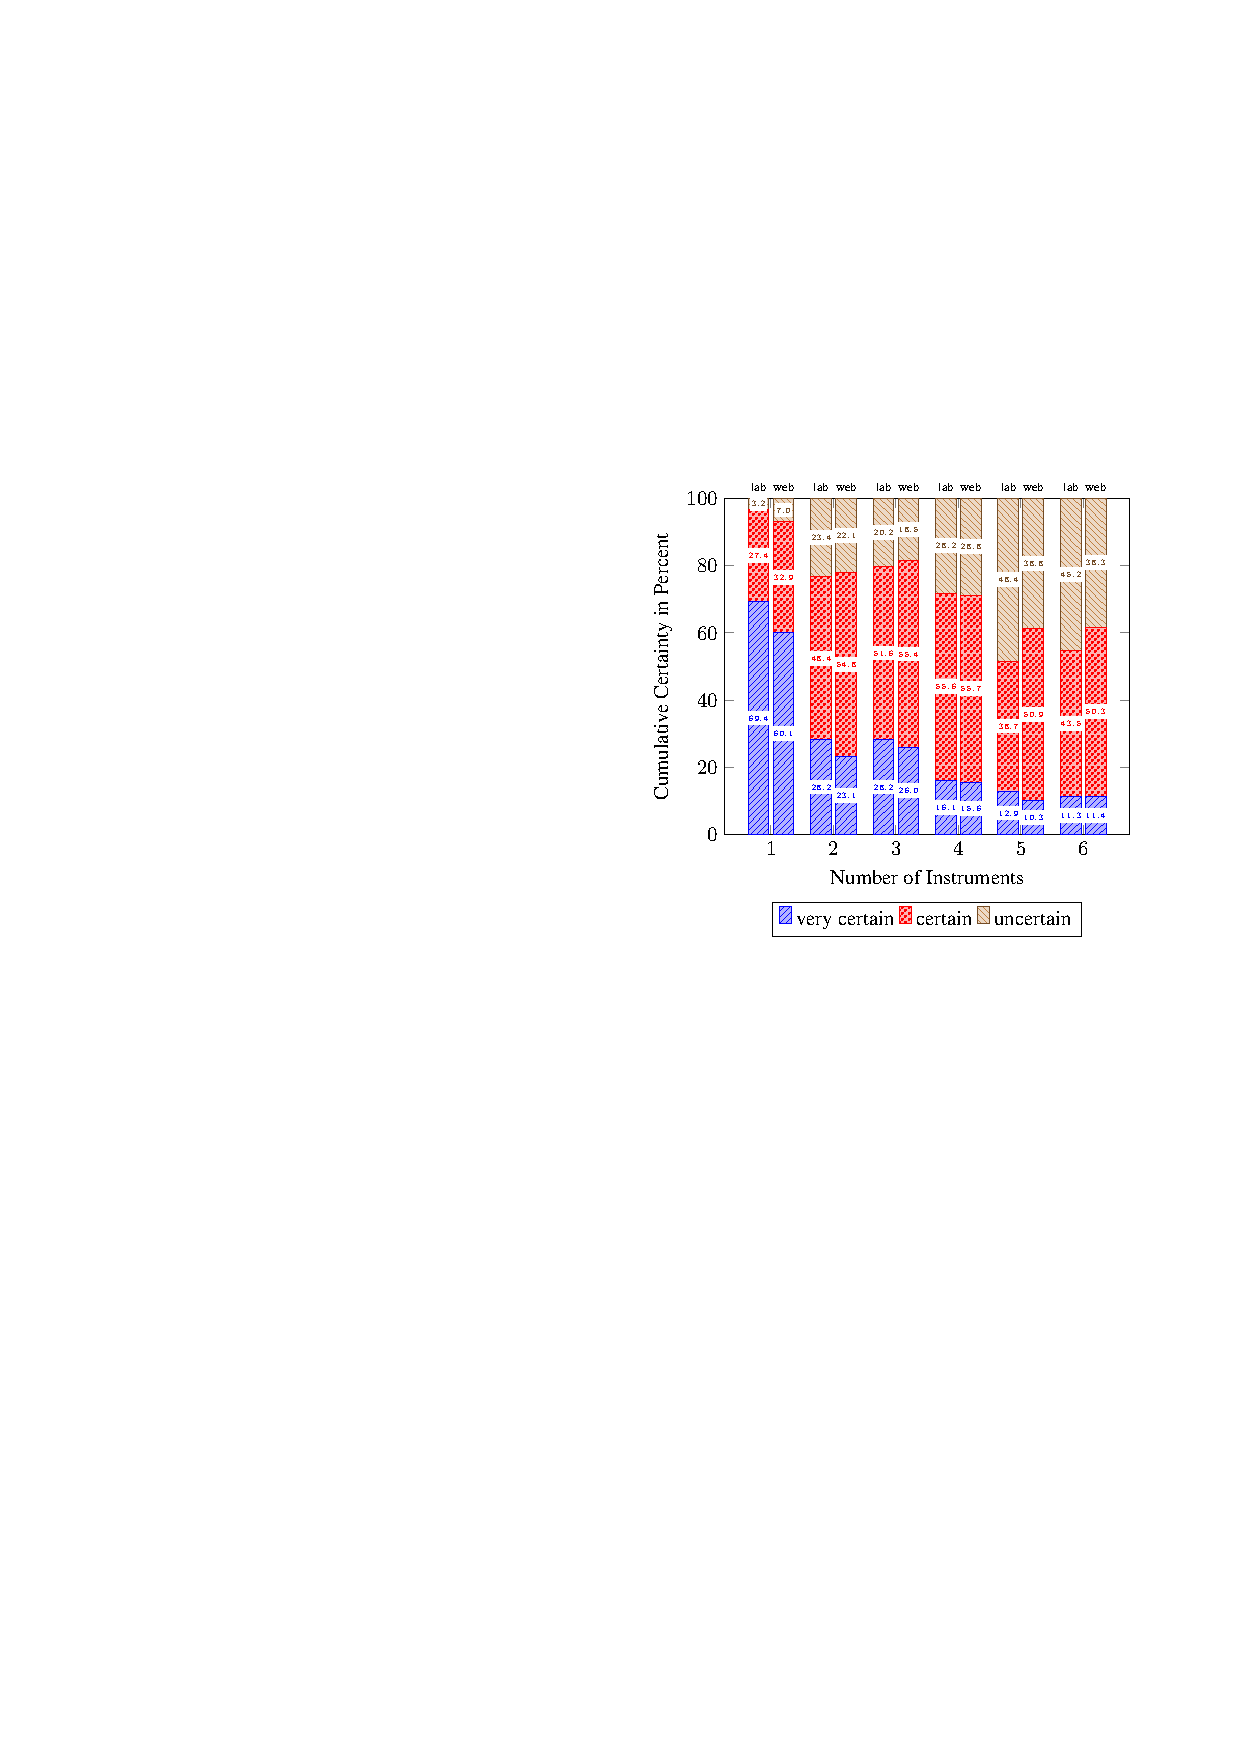
\includegraphics[width=0.45\textwidth]{Chapters/07_Analysis_Experiment/ismir/plotdata/certainty.pdf}
\caption{Differences in certainty between the Internet experiment (web) and laboratory experiment (lab).}
\label{figure:certainty_web_iis}
\end{figure}

To confirm the marginal differences between the Internet experiment and laboratory experiment for $\textit{Dev}_{\mathrm{Abs}}$, a linear regression model was calculated (see Table~\ref{table:lm_absolute_deviation}). Compared to the predictor variable $\textit{Num}_{\mathrm{Inst}}$, the coefficient of $\textit{Environment}$ is very low.
\begin{table}[h]
\center
\scriptsize
\begin{tabular*}{0.45\textwidth}{p{1.5cm}ccccp{0.8cm}}
\toprule[1.5pt]
Coefficient & Estimate & Std. Error & z-value & p-value\\
\midrule
(Intercept) & 0.08535 & 0.02706 & 3.154 & 0.00161\\
$\textit{Num}_{\mathrm{Inst}} = 2$ & 0.17683 & 0.01881 & 9.401  & \textless~2e-16\\
$\textit{Num}_{\mathrm{Inst}} = 3$ & 0.30122 & 0.01881 & 16.014  & \textless~2e-16\\
$\textit{Num}_{\mathrm{Inst}} = 4$ & 1.02154 & 0.01881 & 54.309  & \textless~2e-16\\
$\textit{Num}_{\mathrm{Inst}} = 5$ & 1.67967 & 0.01881 & 89.297  & \textless~2e-16\\
$\textit{Num}_{\mathrm{Inst}} = 6$ & 2.56667 & 0.01881 & 136.453  & \textless~2e-16\\
$\textit{Environment} = \textrm{`}web\textrm{'}$ & 0.05481 & 0.02482 & 2.208  & 0.02724\\
\midrule
\multicolumn{5}{l}{Residual standard error: 0.6597 on 14753 degrees of freedom}\\
\multicolumn{5}{l}{Multiple R-squared: 0.6603,	Adjusted R-squared: 0.6602}\\
\multicolumn{5}{l}{F-statistic:  4779 on 6 and 14753 DF,  p-value: \textless~2.2e-16}\\
\bottomrule[1.5pt]
\end{tabular*}
\caption{Linear regression model for $\textit{Dev}_{\mathrm{Abs}}$ calculated from the data obtained by the Internet experiment and the laboratory experiment.}
\label{table:lm_absolute_deviation}
\end{table}

Another response variable that was obtained from the participants was the certainty of their estimation. Figure~\ref{figure:certainty_web_iis} depicts the certainty values for the Internet experiment and the laboratory experiment.


For testing whether the environment has a significant influence on the certainty of the participants ($\textit{Certainty}$), a cumulative link model (also called ordered regression model) was calculated\cite{Christensen2012}. The cumulative link model is used since $\textit{Certainty}$ is an ordered dependent variable with the possible values `uncertain', `certain' and `very certain'. The predictor variables for the ordered regression model are $\textit{Num}_{\mathrm{Inst}}$ and $\textit{Environment}$. In Table~\ref{table:olr_both} is the cumulative link model for $\textit{Certainty}$ described.
\begin{table}[t]
\center
\scriptsize
\begin{tabular*}{0.45\textwidth}{cccccc}
\toprule[1.5pt]
Coefficient & Estimate & Std. Error & z-value & p-value\\
\midrule
$\textit{Num}_{\mathrm{Inst}} = 2$ & -1.61273 & 0.05744 & -28.078  & \textless~2e-16\\
$\textit{Num}_{\mathrm{Inst}} = 3$ & -1.43164 & 0.05701 & -25.114  & \textless~2e-16\\
$\textit{Num}_{\mathrm{Inst}} = 4$ & -2.02315 & 0.05804 & -34.858  & \textless~2e-16\\
$\textit{Num}_{\mathrm{Inst}} = 5$ & -2.47933 & 0.05901 & -42.013  & \textless~2e-16\\
$\textit{Num}_{\mathrm{Inst}} = 6$ & -2.43573 & 0.05900 & -41.283  & \textless~2e-16\\
$\textit{Environment} = \textrm{`}web\textrm{'}$ & -0.01008 & 0.07355 & -0.137  & 0.891\\
\midrule
\multicolumn{5}{l}{Threshold coefficients:}\\
& Estimate & Std. Error & z-value &\\
$uncertain|certain$ & -2.90465 & 0.08434 & -34.441  &\\
$certain|very certain$ & -0.41072 & 0.08090 & -5.077  &\\
\multicolumn{5}{l}{AIC: 28242.52}\\
\bottomrule[1.5pt]
\end{tabular*}
\caption{Logit cumulative link model of certainty that was calculated from the data obtained by the Internet experiment and the laboratory experiment.}
\label{table:olr_both}
\end{table}
Same as $\textit{Resp}_{\mathrm{Correct}}$, the environment of the experiment has no significant influence on the dependent variable $\textit{Certainty}$. Considering the number of participants and the comparable low coefficient, the environment had a very low influence on $\textit{Certainty}$.

\vspace{-0.1in}
\section{Discussion}\label{sec:discussion}

Regarding the ability of estimating the number of instruments, the web experiment confirmed the results of the laboratory experiment\cite{Stoter2013}. Both experiments share the same outcome: The probability to correctly estimate up to about three instruments is higher than 50\%.

In our previous result analysis of the laboratory experiment\cite{Stoter2013} we set the focus on the differences between musicians and non-musicians. Between the Internet experiment and the laboratory experiment, slightly different results were obtained when looking into how musicians and non-musicians performed (Figure~\ref{figure:error_probability_iis_vs_web}). In the laboratory experiment musicians performed much better compared to non-musicians than in the Internet Experiment. One reason seems to be that in the laboratory experiment 74.2\% of the musicians had also a professional background in audio. In the Internet experiment only 27.5\% of the musicians had a professional background in audio. Since audio professionals more often have to detect hardly audible differences in audio files they are more trained in this field. As mentioned before, being a musician in our context does just mean that the participant plays an instrument without any information about his expert level or the time he or she spends on practicing.

When examining the responses for items with the same number of instruments being played back, noticeable differences between the genres were found. For the stimuli with $\textit{Num}_{\mathrm{Inst}} \le 4$ the mean of $\textit{Resp}_{\mathrm{Correct}}$ was $53.0\%$ and for non-classical items $62.5\%$. Since the experiment was not designed for testing classical versus non-classical items, we cannot make definitive statements about whether humans are better in estimating instruments for a specific music genre. Moreover, we did not address this issue in our result analysis.

One of the main reasons for conducting the experiment was to find out which influence the Internet environment has on the results. All three regression models which included data of both experiments (Table \ref{table:data_both_lm}, \ref{table:lm_absolute_deviation} and \ref{table:olr_both}) revealed that the Internet environment had only very minor effects on the results. Moreover, despite the large number of participants in both experiments, the predictor variable $\textit{Environment}$ was even not significant in two out of three regression models.

It is often recommended to use headphones instead of loudspeakers for Internet experiments. From the relative low average marginal effect of $\textit{Setup}$ (Table~\ref{table:data_web_lm}), it can be derived that the type of the setup had only minor effects on the results of the Internet experiment.

Surprising was the small number of participants who had to be screened. We excluded 27 participants since they gave at least one non-serious response which is about 2.3\% (1195 participants remained after excluding all trials which were not the first ones). Most of these excluded participants responded with either very high numbers (e.~g. 99) or responded with zeros for their estimated number of instruments being played. We assume that especially participants who responded with zero only wanted to get an impression of the experiment.


% The analysis of certainty revealed how difficult the task of estimating the number of instruments is: For up to three instruments the majority of the participants tend to estimate their level on certainty reliably. In more than half of the responses the participants still felt certain or very certain for items of five and six instruments. which gives another indication for the proposed upper limit of three instruments.

\section{Conclusion}\label{sec:conclusion}
The Internet experiment presented in this paper confirmed the results of a previous laboratory experiment that humans are able to correctly estimate up to around three instruments in music. Furthermore significant differences in performance between musicians and non-musicians found out by the previous experiment were confirmed.
The comparison between the results of the Internet experiment and laboratory experiment revealed that only minor differences between both environments exist. Using headphones instead of loudspeaker is often held to be important when conducting listening tests over the Internet. In this experiment the audio setup used had only a minor influence on the results.
According to these results, experiments in the fields of music perception or music information retrieval related to our procedure are well suited for being conducted over the Internet.
